\documentclass[../../main.tex]{subfiles}

\begin{document}

\chapter{Quantum many-body framework}

This chapter is dedicated to introducing the necessary tools needed to perform realistic material calculations using DMFT or D$\Gamma$A. We start with the most central objects - the Green's functions - and subsequently assemble a complete framework which enables us to calculate a number of physical properties, e.g. the susceptibility, optical conductivity, superconductivity, pseudogaps and more, that stem from the correlated interplay between electrons or holes. 

\section{Green's functions}

Green's functions are fundamental tools in many-body physics, used to study the properties and behavior of interacting quantum systems. These mathematical objects encode information about the propagation of particles or excitations within a system and serve as the cornerstone for analyzing both equilibrium and nonequilibrium states. In the many-body regime, Green's functions extend beyond single-particle descriptions to include complex interactions among multiple particles. They provide insights into phenomena such as quasiparticle lifetimes, collective excitations and response functions. Specifically, one- and two-particle Green's functions describe the propagation of a single particle and the correlated motion of particle pairs, respectively. Alongside of the mathematical description of Green's function-based expressions, we also provide a pictorial description of the equations using Feynman diagrams. These Feynman diagrams allow us to easily describe interaction processes visually. Lines and vertices within the diagrams indicate particle propagators and interaction vertices, respectively.

In condensed matter physics, we are only interested in finite-temperature effects. Hence it is practical to use the so-called Matsubara formalism\cite{T. Matsubara. “A new approach to quantum-statistical mechanics”} in imaginary time by performing a Wick rotation $t\to -i\tau$\cite{G. C. Wick. “Properties of Bethe-Salpeter Wave Functions”}.

Furthermore, most many-body quantities described in the following are $n$-point (correlation) functions\footnote{Here, $n$ denotes the number of \say{external legs} of the corresponding Feynman diagram.}. These functions typically include a subset of the following parameters for each external leg: (Matsubara) frequency ($\nu$), spin index ($\sigma$), orbital index ($o$), lattice position ($\vv{R}$), momentum ($\vv{k}$) or imaginary time ($\tau$). This introduces a huge amount of dependencies appended to a variable and can be very cumbersome to read through if explicitly written down. Therefore, to increase readability, we follow Ref.~\cite{N. E. Bickers and D. J. Scalapino. “Conserving approximations ...”} and group all indices that are not explicitly written down into a compound index, e.g. $\mathfrak{1}=\{o_1, \sigma_1, \vv{R}_1\}$. If an equation containing spatial or momentum-dependent quantities is written down with a compound index, it applies equally in both real and Fourier space. Furthermore, summing over these compound indices means summing over all individual components they include, with a normalization of $\frac 1\beta$ for frequency sums and $\frac{1}{N_{\vv{k}}}$ for momentum sums, where $\beta=\frac{1}{k_B T}$ is the inverse temperature and $N_{\vv{k}}$ is the total number of reciprocal lattice points. 



After this short introduction, let us dive in by defining the most central quantity, the one-particle Green's function as
\begin{align}
	G_{\mathfrak{12}}=-\mean{\mathcal{T}\left [\hat{c}_{\mathfrak{1}}\hat{c}^{\dagger}_{\mathfrak{2}}\right ]},
\end{align}
where $\hat{c}_{\mathfrak{i}}$ ($\hat{c}^{\dagger}_{\mathfrak{i}}$) are fermionic annihilation (creation) operators which annihilate (create) an electron with parameters $\mathfrak{i}=\{\sigma_i, o_i, \vv{R}_i, \tau_i\}$ in the system. $\mean{\cdot}=\trace{e^{-\beta\hat{\mathcal{H}}}\;\cdot }$ describes the thermal expectation value. Note, that the time evolution operator $e^{i\hat{\mathcal{H}}t}=e^{\hat{\mathcal{H}}\tau}$ is real after performing the Wick rotation to imaginary time and the Boltzmann weight $e^{\beta\hat{\mathcal{H}}}$ describes nothing more than an additional evolution in imaginary time. Lastly, $\mathcal{T}[\cdot]$ is the imaginary time ordering operator, where
\begin{align}
	\mathcal{T}\left [\hat{c}^{(\dagger)}_{\mathfrak{1}}(\tau_1)\hat{c}^{(\dagger)}_{\mathfrak{2}}(\tau_2)\right ]=\Theta(\tau_1-\tau_2)\hat{c}^{(\dagger)}_{\mathfrak{1}}(\tau_1)\hat{c}^{(\dagger)}_{\mathfrak{2}}(\tau_2)-\Theta(\tau_2-\tau_1)\hat{c}^{(\dagger)}_{\mathfrak{2}}(\tau_2)\hat{c}^{(\dagger)}_{\mathfrak{1}}(\tau_1).
\end{align}
The Green's function measures the probability amplitude of a propagation process and reads as a Feynman diagram
\begin{figure}
	\centering
	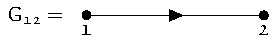
\includegraphics{../../Graphics/Diagrams/one_p_green/one_p_green.pdf}
	\caption{•}
	\label{•}
\end{figure}

\end{document}
